\documentclass[
  journal=small,
  manuscript=mini-article,  % Use a - if you need a space e.g. "research-article"
  year=2023,
  volume=1,
]{odj-journal}

\usepackage{amsmath}
\usepackage[nopatch]{microtype}
\usepackage{booktabs}
\usepackage{threeparttable}
\usepackage{longtable}
\usepackage{lipsum} 
\usepackage{subcaption}
\usepackage[square,sort,comma,numbers]{natbib}
\usepackage[colorlinks]{hyperref}
\hypersetup{
     colorlinks =true,
     linkcolor  =cyan,
     filecolor  =cyan,
     citecolor  =black,      
     urlcolor   =cyan,
}
\usepackage{listings}
\usepackage{color}

\definecolor{dkgreen}{rgb}{0,0.6,0}
\definecolor{gray}{rgb}{0.5,0.5,0.5}
\definecolor{mauve}{rgb}{0.58,0,0.82}

\lstset{frame=tb,
  language=Python,
  aboveskip=3mm,
  belowskip=3mm,
  showstringspaces=false,
  columns=flexible,
  basicstyle={\small\ttfamily},
  numbers=none,
  numberstyle=\tiny\color{gray},
  keywordstyle=\color{blue},
  commentstyle=\color{dkgreen},
  stringstyle=\color{mauve},
  breaklines=true,
  breakatwhitespace=true,
  tabsize=3
}


\title{Nature's SOS: Decoding Civil Protection in Catalonia}

\author{Ot Garcés Ortiz}
\affiliation{MSc Physics of Complex Systems and Biophysics}
\email[Ot Garcés]{ogarceor43@alumnes.ub.edu}

\author{Belén Montenegro}
\affiliation{MSc Physics of Complex Systems and Biophysics}
% \alsoaffiliation{Joint first authors}

\author{Iván Casanovas}
\affiliation{MSc Physics of Complex Systems and Biophysics}

\author{Imma Passaret}
\affiliation{MSc Physics of Complex Systems and Biophysics}
\keywords{rescue; natural enviroment; civil protection plans; incidents; Catalonia} 


\begin{document}
\vspace{-0.5cm}
\begin{abstract}
In the past five to six decades, the frequency of natural disasters has significantly increased, as highlighted by the 2020 Ecological Threat Register (ETR). Public civil protection (CP) organizations must adapt to circumstances caused by climate change and the consequent potential civil threats, and thus, it is of primordial importance analyzing and evaluating the response of those organisms that must guarantee civil protection. The main objective of the project is to give a broad vision on how rescue actions in natural enviroment are correlated to government action on civil protection. In this paper, we show that there are distinct geographical patterns in rescue actions across Catalonia, and that short-time correlations between government CP action and rescue operations are the key to evaluate the response against global threats. We also emphasize the necessity of improving the resolution of date and time data for a more comprehensive and thorough evaluation of these responses.
\end{abstract}
% ----------------------------------------------------- BACKGROUND -----------------------------
\vspace{-1cm}
\section{Background}
The research project aims to identify geographical and temporal correlations between natural environment rescue operations by the Fire Department (FD) and modifications in the legal status of civil protection plans (CPP). The study, conducted between years 2018 and 2022, also explores patterns and biases between incidents reported by the Generalitat de Catalunya and FD rescue operations and changes in legal status of CPP. The project's tasks were divided among team members, with my focus on finding geographical correlations/uncorrelations in FD rescue actions and CPP legal status modifications. This mini-article adresses my contribution to the whole project and includes detailed sections on methodologies (see Sec. \ref{sec:methods}), main results (see Sec. \ref{sec:res}) and some conclusive ideas on my research (see Sec. \ref{sec:conclusions}). \\

The data for this project is sourced from the \textit{Dades Obertes de Catalunya}\footnote{For usage conditions and licenses, see \href{https://governobert.gencat.cat/ca/dades_obertes/llicencia-oberta-informacio-catalunya/}{\textit{Llicència oberta d'ús d'informació Catalunya}}.} portal \cite{dades_obertes}. The primary datasets include "\textit{Actuacions en salvaments al medi natural dels Bombers de la Generalitat}" (identifier \texttt{fsum-2k6e}) \cite{fd_rescue} and "\textit{Registre general de plans de protecció civil de Catalunya}" (identifier \texttt{xqqe-tgav}) \cite{CPP}. The former details natural environment rescue actions by the Generalitat de Catalunya Fire Department, available from 2010 to date, including georeferenced information. This dataset is openly accessible on the \textit{Dades Obertes de Catalunya} portal, provided by \textit{Departament d'Interior} and \textit{Direcció General de Prevenció, Extinció d'Incendis i Salvaments}. The latter dataset records civil protection plans (CPP) approved by the Generalitat de Catalunya, starting from November 22, 1990. Supra-municipal CPPs and those unrelated to natural disasters (e.g., RADCAT, CAMCAT, PLASEQCAT, and PLASEQTA) will be excluded. This dataset is also available on \textit{Dades Obertes de Catalunya} and provided by \textit{Departament d'Interior}. While data collection details are not provided, further information can be found on the portal.\\

Additionally, a dataset from the \textit{Institut Cartogràfic i Geològic de Catalunya (ICGC)} \cite{geo_dades} was used in order to map Catalonia counties. This dataset contains the administrative divisions' geometry as of August 1, 2022, prior to the 2023 map change due to the creation of the new county Lluçanès.

\section{Methods}\label{sec:methods}
Data for the project was directly downloaded from the portal \textit{Dades Obertes de Catalunya} in \texttt{.csv} format and loaded into our group's GitHub repository Jupyter Notebooks \cite{github_repo}. The re-used data was clean and required minimal modifications. To align with our group's analysis timeframe (2018-2022), I filtered the datasets accordingly, with additional date standardization for the CPP dataset. Specifically, for the "\textit{Registre general de plans de protecció civil de Catalunya}" dataset, I excluded CPP unrelated to natural environments or directly linked to human action (RADCAT, CAMCAT, etc.). Further modifications included filtering CPP names for essential plan type information, dropping unused columns, and creating new memory-allocated dataframes for clarity in the analysis.\\

To analyze geographical correlations between Fire Department rescue actions and changes in legal status of CPP, I grouped both datasets by county within the specified time window. Calculating the total counts, I noticed that the dataset "\textit{Actuacions en salvaments al media natural dels Bombers de la Generalitat}" included FD actions outside of Catalonia, which I dropped to restrict the analysis. After identifying the top five counties with highest count of rescue actions and CPP modifications, I merged the grouped dataframes with additional map geometry information. Using \texttt{geopandas}, I created geographical plots highlighting the top counties in the corresponding heatmaps (see table Tab. \ref{tab:tab1} and figure Fig. \ref{fig:fig1} in section Sec. \ref{sec:res}).\\

Finally, Osona and Baix Llobregat were selected for a specific study due to their qualitative different behavior. To focus on these counties, I further filtered the data. I also carried some data exploration with the aim to standardize the nomenclature of rescue operations. For CPP data, a new column indicating the corresponding year was added. Then, I grouped the dataframes for Osona and Baix Llobregat by year, rescue action typology, and CPP typology. Bar plots were generated for both number of rescue actions and modifications in legal status of CPP by year, hued by rescue action and CPP typology (see figures Figs. \ref{fig:sub1}-\ref{fig:sub2}).\\

As previously mentioned, the code used for data processing is openly accessible in our group's GitHub repository \cite{github_repo}. The results, which will be discussed in the next section, are well documented in the corresponding Jupyter Notbook for easy follow-up and reproduction by anyone.

\section{Results}\label{sec:res}
To identify geographical patterns and correlations in our data, we adopted a direct approach $-$calculating the total number of rescue actions and modifications in CPP by county and examining the geographical heatmap of these totals. Following the methodology outlined in the previous section, we identified the top five counties with the highest counts of rescue actions and modifications in the legal status of CPP. The results are as follows:


\begin{longtable}{p{2.5cm}p{2.5cm}p{2.5cm}p{2.5cm}}
  \caption{Counties with most rescue action and modification on legal status of CPP counts between 2018 and 2022.}\label{tab:tab1}\\
  \toprule
  \textbf{Dataset} & \textbf{County} & \textbf{$\#$ Counts} \\
  \midrule
  \endhead
  \midrule
  \endfoot
  Rescue actions & Baix Llobregat & 527 \\
   & Vallès Occidental & 517 \\
   & Val d'Aran & 500 \\
   & Ripollès & 479 \\
   & Berguedà & 417 \\
  \midrule
  CPP & Osona & 138 \\
   & Noguera & 85 \\
   & Alt Penedès & 84 \\
   & Bages & 82 \\
   & Baix Empordà & 82 \\
  \bottomrule
\end{longtable}
Table Tab. \ref{tab:tab1} shows little difference in rescue action counts across regions. However, a notable gap appears in modifications to CPP legal status, with Osona having around 50 more instances than other counties. Geographical plots in figure Fig. \ref{fig:fig1} further illustrate these findings.

\begin{figure}[hbt!]
\centering
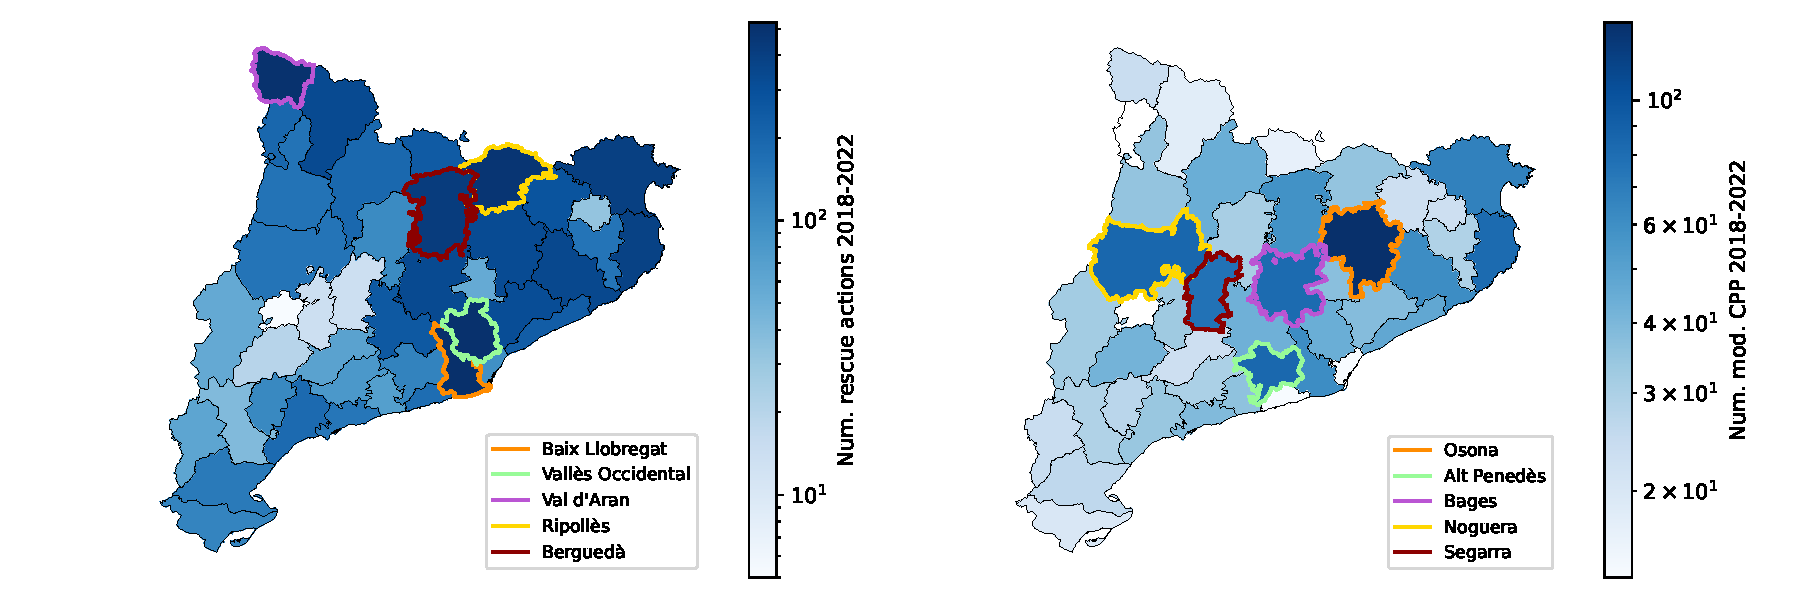
\includegraphics[width=1\linewidth]{../figures/merged_maps_plot}
\caption{Heatmaps displaying the total rescue actions and CPP modifications by county. The left shows a geographical plot of rescue actions, and the right depicts changes in CPP count. Both highlight counties with the highest counts from table Tab. \ref{tab:tab1}.}
\label{fig:fig1}
\end{figure}
From figure Fig. \ref{fig:fig1}, we find that counties with the highest rescue actions are, a priori, not geographically correlated with those having the most changes in CPP legal status, as indicated in Table Tab. \ref{tab:tab1}. We also note that there is a tendency for the accumulation of rescue actions in the northern region of Catalonia, possibly due to mountain rescues in the Pyrenees and pre-Pyrenees, though this is beyond the scope of my analysis but my colleague Imma Passaret will provide more details. Lastly, we note that Osona and Baix Llobregat exhibit qualitative differences: Baix Llobregat has the most rescue actions but a moderate number of CPP legal status changes, while Osona has a substantial number of changes in CPP and a high number of rescue actions. Separate analysis for Osona and Baix Llobregat by year are presented in figures Figs. \ref{fig:sub1}-\ref{fig:sub2}.

\begin{figure}
\centering
\begin{subfigure}{0.47\textwidth}
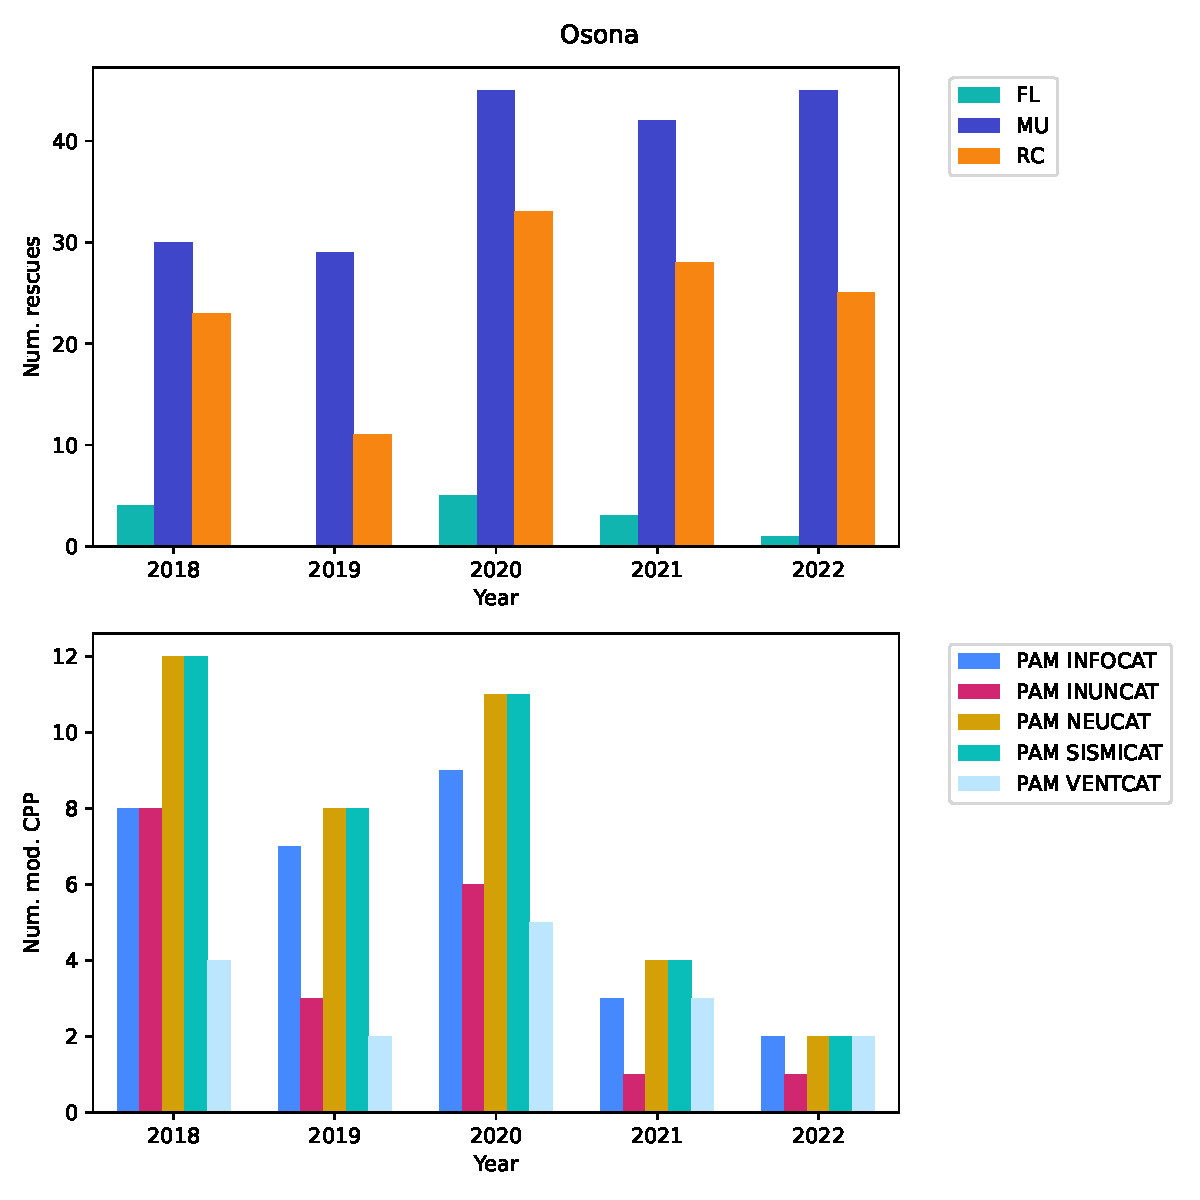
\includegraphics[width=\textwidth]{../figures/combined_plot_osona.pdf}
\caption{}
\label{fig:sub1}
\end{subfigure}\hskip1ex
\begin{subfigure}{0.47\textwidth}
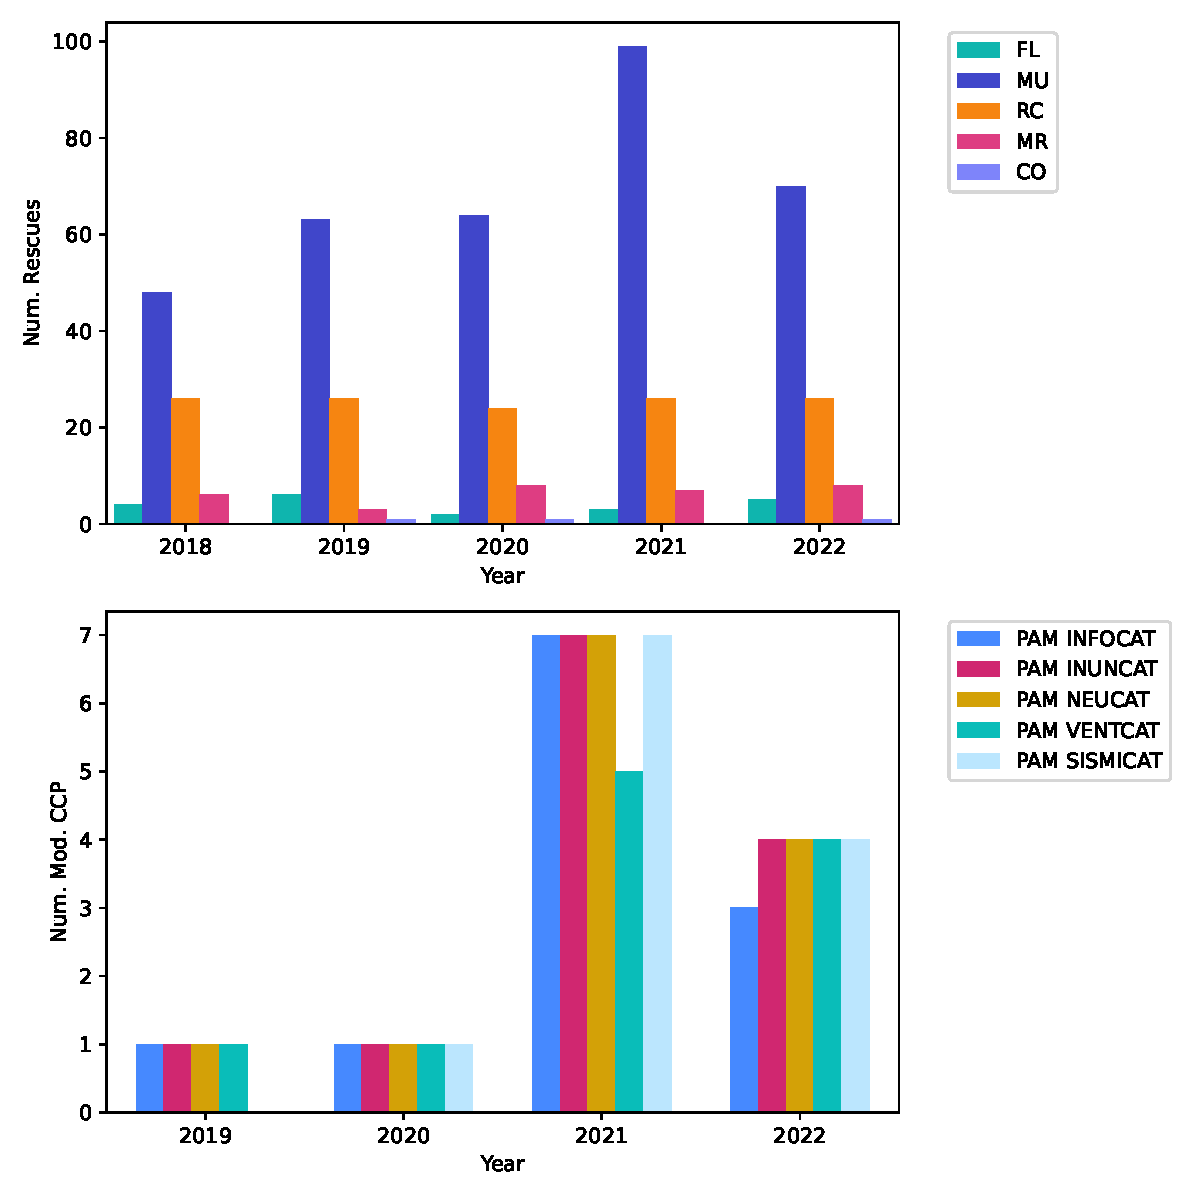
\includegraphics[width=\textwidth]{../figures/combined_plot_baix_llobregat.pdf}
\caption{}
\label{fig:sub2}
\end{subfigure}
\caption{Barplots showing the total count of rescue actions and changes in legal status of CPP per year hued by rescue and CPP typology. Subplot (a) corresponds to data for Osona whilst subplot (b) corresponds to data for Baix Llobregat. For Baix Llobregat, no data was provided in the year 2018. Codes for rescue actions FL, MU, RC, MR and CO correspond to fluvial, mountain, research, maritime and cave rescues, respectively. Codes for CPP belong to different types of CPP.}
\end{figure}
As previously mentioned, we observe a distinct qualitative behavior: in Osona, rescue actions appear somewhat uncorrelated, as peaks in changes of CPP legal status do not align with rescue actions. Contrarily, in Baix Llobregat, there is a well-defined peak in both rescue actions and CPP changes in the year 2021. This suggests the idea that the evaluation of the response of agencies reponsible for civil protection is encoded in those short-time scale correlations.

\section{Conclusions / Discussion}\label{sec:conclusions}
One of the main findings from our study is that, at a large time scale analysis, there appears to be no inherent correlation between rescue actions and changes in the legal status of CPP. In many cases, rescue actions seem to be responses to individual emergencies rather than indicators of global civil threats or major civil protection actions. However, short-term correlations are evident in certain cases, such as in Baix Llobregat.

On the other hand, the geographical heatmap of rescue actions by county reveals a notable concentration in the northern region of Catalonia, particularly associated with mountain environment rescue actions, as highlighted in the analysis by our colleague Imma Passaret. In contrast, the heatmap depicting changes in the legal status of CPP suggests that these rescue actions are not directly linked to civil protection actions.

Finally, our study indicates that short-time correlations between rescue actions and modifications in the legal status of CPP serve as a means to test and evaluate the response of public agencies to global threats. To conduct a more comprehensive evaluation of public agency responses in civil protection, there is a need to improve the resolution of date data, potentially moving towards date and time resolution. Future research could further explore and evaluate the responses of public agencies in civil protection, getting involved in these aspects in greater detail.



\bibliographystyle{acm}
\bibliography{bibliography}

\end{document}